\documentclass[11pt,a4paper]{article}
\usepackage{geometry}
\usepackage{graphicx}
\usepackage{amsmath}
\usepackage{listings}
\usepackage{xcolor}
\usepackage{float}
\usepackage{caption}
\usepackage{subcaption}
\usepackage{textcomp}
\usepackage[utf8]{inputenc}

\geometry{margin=2.5cm}

% MATLAB code style
\lstdefinestyle{matlab}{
    language=Matlab,
    basicstyle=\small\ttfamily,
    keywordstyle=\color{blue},
    commentstyle=\color{green!60!black},
    stringstyle=\color{red},
    numberstyle=\tiny\color{gray},
    breaklines=true,
    frame=single,
    backgroundcolor=\color{gray!10},
    numbers=left,
    numbersep=5pt,
    showstringspaces=false,
    tabsize=2
}

\title{EN3563 Robotics Laboratory Experiment 01\\
Answer Sheet}
\author{Index No: 220148G \hspace{3cm}}
\date{}

\begin{document}

\maketitle

\section{MATLAB Code for Tasks 3.1 to 3.5}

\begin{lstlisting}[style=matlab, caption={Task 1 MATLAB Code (3.1-3.5)}]
clear; close all; clc;

% 3.1 - Visualize default 2D coordinate frame {0}
figure; hold on; grid on; axis([-4 7 -2 7]);
trplot2(eye(3), 'frame','0');

% 3.2 - Plot point p with position vector [5 6]^T in frame {0}
p_in_0 = [5;6];
quiver(0,0, p_in_0(1), p_in_0(2), 'b');
text(p_in_0(1)-0.4, p_in_0(2)-0.2, 'p', 'FontSize', 12, 'Color', 'b');

% 3.3 - Rotate frame {0} counterclockwise by 45 degrees
R_1_in_0 = rot2(45*pi/180);
T_1_in_0 = [R_1_in_0 [0;0]; 0 0 1];
tranimate2(eye(3), T_1_in_0, 'cleanup', true);
trplot2(T_1_in_0, 'frame','1', 'color','r');

% Find p in frame {1}
p_in_1 = inv(R_1_in_0) * p_in_0;

% 3.4 - Point q with position vector [-3 2]^T in frame {1}
q_in_1 = [-3;2]; 
q_in_0 = R_1_in_0 * q_in_1;
quiver(0,0, q_in_0(1), q_in_0(2), 'r');
text(q_in_0(1)-0.2, q_in_0(2)+0.1, 'q', 'FontSize', 12, 'Color', 'r');

% 3.5 - Apply 68 degree counterclockwise rotation to p
R68 = rot2(68,"deg");           
r_in_0 = R68 * p_in_0;          
quiver(0,0, r_in_0(1), r_in_0(2), 0, 'Color','g');
text(r_in_0(1), r_in_0(2), '  r', 'Color','g','FontWeight','bold');
\end{lstlisting}

\section{Final Output MATLAB Figure for Operations 3.1 to 3.5}

\begin{figure}[H]
    \centering
    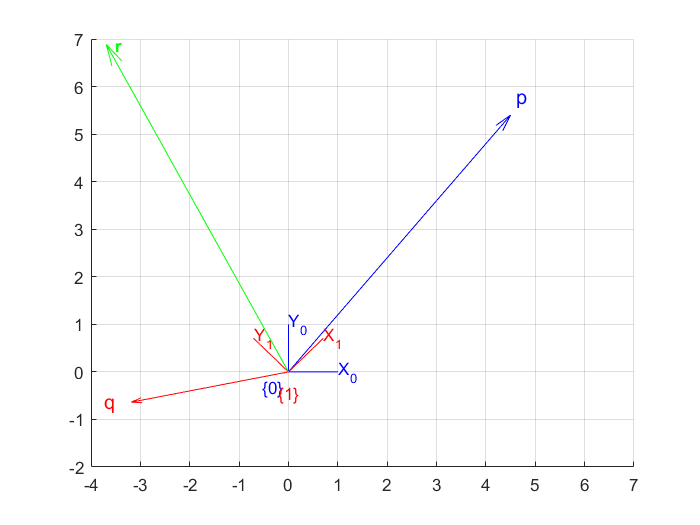
\includegraphics[width=0.8\textwidth]{task_1.png}
    \caption{2D Coordinate frames and vector transformations showing frame \{0\} (blue), frame \{1\} rotated 45° (red), point p (blue arrow), point q (red arrow), and rotated point r (green arrow)}
\end{figure}

\section{$p^1$ for Task 3.3}

To find point $p$ represented in frame $\{1\}$, we use the inverse transformation:

$$p^1 = (R_1^0)^{-1} \cdot p^0 = (R_1^0)^T \cdot p^0$$

Where $R_1^0 = \begin{bmatrix} 
\cos(45^\circ) & -\sin(45^\circ) \\ 
\sin(45^\circ) & \cos(45^\circ) 
\end{bmatrix} = \begin{bmatrix} 
0.7071 & -0.7071 \\ 
0.7071 & 0.7071 
\end{bmatrix}$

$$p^1 = \begin{bmatrix} 
0.7071 & 0.7071 \\ 
-0.7071 & 0.7071 
\end{bmatrix} \begin{bmatrix} 5 \\ 6 \end{bmatrix} = \begin{bmatrix} 7.7782 \\ 0.7071 \end{bmatrix}$$

\section{$R_1^0$ for Task 3.7}

The rotation matrix $R_1^0$ is obtained by sequential rotations:
\begin{enumerate}
    \item Rotate about X axis by +15\textdegree
    \item Rotate about current Y axis by +25\textdegree  
    \item Rotate about current Z axis by +35\textdegree
\end{enumerate}

$$R_1^0 = R_x(15^\circ) \cdot R_y(25^\circ) \cdot R_z(35^\circ) = \begin{bmatrix}
0.7424 & -0.5198 & 0.4226 \\
0.6436 & 0.7285 & -0.2346 \\
-0.1859 & 0.4462 & 0.8754
\end{bmatrix}$$

\section{MATLAB Code for Tasks 3.6 to 3.9}

\begin{lstlisting}[style=matlab, caption={Task 2 MATLAB Code (3.6-3.9)}]
clear; close all; clc;

% 3.6 - Visualize default 3D coordinate frame {0}
figure;
hold on; grid on; view(3);
axis([-1 2 -1 2 -1 2]);
trplot(eye(4), 'frame', '0');

% 3.7 - Sequential rotations: X(+15 deg), Y(+25 deg), Z(+35 deg)
Rx = rotx(15,'deg');
Ry = roty(25,'deg');   
Rz = rotz(35,'deg');   
R1_0 = Rx * Ry * Rz;
tranimate(eye(3), R1_0,'axis',[-1 2 -1 2 -1 2], 'color','r');
trplot(R1_0, 'frame','1', 'color','r', 'arrow');
disp('R1_0 ='); disp(R1_0);

% 3.8 - Find default roll-pitch-yaw definition
testR = R1_0;
rpy_default = tr2rpy(testR);              % default sequence
rpy_zyx     = tr2rpy(testR, 'zyx');
rpy_xyz     = tr2rpy(testR, 'xyz');
rpy_yxz     = tr2rpy(testR, 'yxz');

fprintf('tr2rpy default (rad): [%.4f %.4f %.4f]\n', rpy_default);
fprintf('tr2rpy zyx (rad): [%.4f %.4f %.4f]\n', rpy_zyx);
fprintf('tr2rpy xyz (rad): [%.4f %.4f %.4f]\n', rpy_xyz);
fprintf('tr2rpy yxz (rad): [%.4f %.4f %.4f]\n', rpy_yxz);

% 3.9 - Convert given rotation matrix to roll-pitch-yaw angles
R = [ 0.8138  0.0400  0.5798;
      0.2962  0.8298 -0.4730;
     -0.5000  0.5567  0.6634 ];

rpy_deg = tr2rpy(R, 'zyx', 'deg');      % [roll psi, pitch theta, yaw phi]
psi = rpy_deg(1);  theta = rpy_deg(2);  phi = rpy_deg(3);

fprintf('RPY (deg): roll psi = %.4f deg, pitch theta = %.4f deg, yaw phi = %.4f deg\n', ...
        psi, theta, phi);

% Verification: Opposite conversion
R_from_rpy = rpy2r([psi theta phi], 'zyx', 'deg');
fprintf('||R - rpy2r||_F = %.3e\n', norm(R - R_from_rpy, 'fro'));

% Verification: Product of basic rotation matrices
R_basic = rotz(phi, 'deg') * roty(theta, 'deg') * rotx(psi, 'deg');
fprintf('||R - (Rz*Ry*Rx)||_F = %.3e\n', norm(R - R_basic,'fro'));
\end{lstlisting}

\section{Final Output MATLAB Figure for Operations 3.6 to 3.9}

\begin{figure}[H]
    \centering
    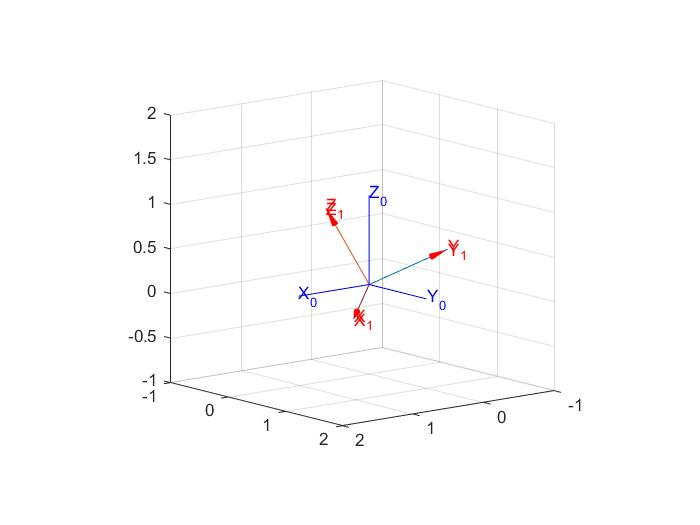
\includegraphics[width=0.8\textwidth]{task_2.jpg}
    \caption{3D Coordinate frames showing default frame \{0\} (blue) and rotated frame \{1\} (red) after sequential rotations about X, Y, and Z axes}
\end{figure}

\section{Default Roll-Pitch-Yaw Angle Definition}

Based on the MATLAB Robotics Toolbox analysis, the default roll-pitch-yaw angle definition is:
\begin{itemize}
    \item \textbf{Default sequence}: ZYX (same as 'zyx' option)
    \item \textbf{Convention}: Intrinsic rotations (body-fixed axes)
    \item \textbf{Order}: 
    \begin{enumerate}
        \item Roll ($\psi$): rotation about X-axis
        \item Pitch ($\theta$): rotation about Y-axis  
        \item Yaw ($\phi$): rotation about Z-axis
    \end{enumerate}
\end{itemize}

The transformation is: $R = R_z(\phi) \cdot R_y(\theta) \cdot R_x(\psi)$

\section{Results for Task 3.9}

For the given rotation matrix:
$$R = \begin{bmatrix}
0.8138 & 0.0400 & 0.5798 \\
0.2962 & 0.8298 & -0.4730 \\
-0.5000 & 0.5567 & 0.6634
\end{bmatrix}$$

The roll-pitch-yaw angles are:

$$\psi: \boxed{40.0021^\circ} \quad \theta: \boxed{29.9999^\circ} \quad \phi: \boxed{20.0001^\circ}$$

\textbf{Verification:}
\begin{itemize}
    \item Reconstruction error: $||R - \text{rpy2r}||_F = 8.286 \times 10^{-5}$
    \item Basic matrices error: $||R - (R_z \cdot R_y \cdot R_x)||_F = 8.286 \times 10^{-5}$
\end{itemize}

Both verification methods confirm the accuracy of the conversion.

\end{document}